\chapter{Esquema de segmentación propuesto}\label{chapter:metodos}
Este capítulo tiene por objetivo presentar el esquema de segmentación propuesto en este trabajo.  El mismo está basado en la combinación de un algoritmo de Fuzzy C-Means con un esquema de Modelos Deformables. Esta integración permite incorporar fácilmente la información de distintos descriptores extraídos a partir de una imagen al método de Superficies Activas, y al mismo tiempo establecer restricciones espaciales sobre la malla obtenida utilizando Fuzzy C-Means.
 
La primera etapa de esta propuesta, basada en Fuzzy C-Means se inicializa con la imagen original, indicando la cantidad de regiones que se desean segmentar en la misma (clusters). El resultado es un mapa probabilístico por cluster, que indica para cada punto de la imagen, su probabilidad de pertenencia al mismo.

A partir de estos mapas probabilísticos, y luego de seleccionar la región de interés, se realiza un umbralado y extracción del contorno del objeto para obtener una malla inicial, que es utilizada luego como entrada para el esquema de Superficies Activas. El algoritmo toma la malla de entrada y la deforma utilizando para ello utilizando para ello la matriz de probabilidades previamente obtenida por Fuzzy C-Means.

En la siguiente sección (\ref{section:descripcion_general}) se resume, en términos generales, el esquema propuesto. En la Sección \ref{section:segmentacion_fuzzy} se hace especial hincapié en el algoritmo de Fuzzy C-Means, en la Sección \ref{section:extraccion_de_mallas} se explican los pasos para realizar la extracción de la malla de superficie, mientras que en la Sección \ref{section:modelos_deformables} se detalla el algoritmo de Snakes utilizado.

\section{Descripción general}\label{section:descripcion_general}
El esquema de segmentación propuesto es un pipeline de procesamiento dividido en etapas, en donde la salida de cada una es la entrada de la siguiente (Figura \ref{fig:esquema_de_segmentacion}).


\begin{figure}[H]
	\centering
	\includegraphics[scale=0.4]{images/pipeline_de_segmentacion.jpg}
	\caption{Esquema de segmentación}
	\label{fig:esquema_de_segmentacion}
\end{figure}

Para la primera etapa se utiliza el algoritmo de Fuzzy C-Means (Sección \ref{section:segmentacion_fuzzy}). Este enfoque permite, dada una imagen tridimensional y el número $c$ de regiones en las que se espera se divida la misma, obtener una serie de mapas probabilísticos que describen con cuánta probabilidad un punto pertenece o no a una determinada región de interés. A partir de estos mapas se realizan una serie de operaciones una serie de operaciones mediante las cuales se obtiene un volumen inicial, binario y uniforme, de cada segmento. Estos volúmenes son sometidos posteriormente a un método de extracción de mallas, mediante el cual se construye una geometría basada en triángulos que recubre completamente a cada región (Sección \ref{section:extraccion_de_mallas}). Finalmente, una de las mallas es escogida por el usuario, para ser refinada utilizando un esquema de Modelos Deformables (Sección \ref{section:modelos_deformables}). El resultado es una superficie suave que recubre a la región de interés y que se asemeja significativamente a la estructura real del objeto.

\section{Segmentación por Fuzzy C-Means}\label{section:segmentacion_fuzzy}
\chapter{Fuzzy C-Means}
\section{Introducción}
\label{Introduccion}

Como se explicó anteriormente, la etapa inicial del enfoque de segmentación propuesto está basado en el método de Fuzzy C-Means. Este algoritmo de clustering no supervisado, que fue introducido por Dunn en 1973 \citep{dunn1973fuzzy} y extendido luego en \citep{bezdek1984fcm}, permite obtener segmentaciones difusas agrupando elementos similares en clusters. Un cluster es un conjunto de elementos que son afines entre sí, de acuerdo a algún criterio. Una de las principales desventajas de los algoritmos de clustering tradicionales radica en que los mismos asumen que cada elemento pertenece inequívocamente a un cluster, ignorando si existe o no alguna similitud con los demás miembros de otros clusters \citep{full1982fuzzy}.
 
Una manera de modelar esta similitud fue introducida en \citep{zadeh1965fuzzy}, y consiste en representar la similitud de los puntos que se desean agrupar con una función cuyos valores están entre cero y uno. Basado en esta propuesta, y a diferencia de K-Means, en donde cada elemento pertenece o no a un cluster de manera inequívoca, en el enfoque de Fuzzy C-Means cada elemento posee una cierta probabilidad de pertenencia a cada uno de los clusters. Este agrupamiento se obtiene minimizando iterativamente una función de costo que depende de la similitud de los elementos de un cluster respecto al centroide del mismo. El centroide es el vector característico de un clúster, obtenido como el promedio de los vectores de características de los puntos que pertenecen al mismo. A cada clúster le corresponde un único centroide, que varía conforme se le incorporan o se le quitan puntos.

Fuzzy C-Means requiere como entrada un vector de características por cada uno de los puntos que se desean clusterizar, y el número de clusters en los que se quiere dividir la imagen. El algoritmo asigna cada punto a una categoría con una cierta probabilidad de pertenencia. Más formalmente, sea $ X = (x_1, x_2, ..., x_n)$ una imagen de $N$ puntos a ser particionados en $c$ regiones, en donde cada $x_i$ representa el vector de características del $i$-ésimo punto. El algoritmo asigna cada punto a una clase a través de la minimización iterativa de una función de costo, definida como:

\[\label{eq:solve} J = \sum_{j=1}^{N} \sum_{i=1}^{c} u_{ij}^m \lVert x_j- v_i \rVert^2\]

donde $u_{ij}$ representa la pertenencia de un punto $x_j$ al cluster $i$, $v_i$ es el centroide del cluster , $\lVert \rVert$ es la distancia euclídea entre los puntos y $m$ es una constante. Esta constante controla el nivel de difusión de la clusterización resultante \citep{chuang2006fuzzy} y toma valores entre $1 < m < \infty$. No existen en la literatura estudios teóricos o computacionales que distingan un m óptimo, aunque un análisis empírico permite determinar que el incremento del valor de m tiende a degradar la pertenencia. El rango de valores útiles, de acuerdo a varios experimentos, corresponde a valores entre $1$ y $30$ aproximadamente. Para la mayor parte de las imágenes analizadas, $1,5 < m < 3,0$ permite obtener buenos resultados \citep{bezdek1984fcm}. Sin embargo, el valor utilizado en nuestros estudios es de m = 2, ya que todos los experimentos realizados en la bibliografía consultada lo utilizan \citep{caldairou2011non, yang2005fuzzy, chuang2006fuzzy}.

La función de costo tiene por objetivo asignar probabilidades altas de pertenencia de un punto $j$ a un cluster $i$ si su vector característico asociado $x_j$ es similar al centroide $v_i$. Esta similitud entre vectores es cuantificada midiendo la distancia euclídea entre ambos en el espacio de características: si el vector de características es muy disímil respecto al centroide del cluster de estudio, la distancia euclídea entre ambos será alta; si los vectores son similares, la distancia será menor. El resultado del proceso de segmentación es una matriz de pertenencias o mapas probabilísticos, y una lista con los centroides de cada una de las regiones.



\begin{algorithm}[H]
Inicializar $c$ \tcc*[r]{cantidad de clusters}
Inicializar $n$ \tcc*[r]{nivel de difusión}
Inicializar $\epsilon$\;
Inicializar $U = u_{ij}$ \tcc*[r]{matriz  de pertenencias inicial}
$b = 0$\;
\While{$\delta > \epsilon$ | $b <> looplimit$}{
Calcular los centroides $v_{i}^{(b)}$ utilizando $U^{(b)}$\;
Calcular pertenencia de los voxels $U_{b+1}$\;
Calcular $\delta = $\;
$b = b+1$\
}
\caption{Pseudocódigo del algoritmo de Fuzzy C-Means}
\label{lst:fcm-alg}
\end{algorithm}


Como se describe en el pseudocódigo \ref{lst:fcm-alg}, el algoritmo trabaja de manera iterativa, minimizando la función de costo $U$. En cada iteración se calcula un valor delta ($\delta$) que es la diferencia entre el costo de la iteración anterior y la actual. Cuando $\delta$ es menor a la cota de un epsilon ($\epsilon$) predefinido, se considera que el algoritmo ha convergido. En algunas condiciones puede ocurrir que no llegue a la convergencia o que no lo haga en un número práctico de iteraciones. Por este motivo, se añade un mecanismo de control que consiste en limitar la cantidad máxima de iteraciones. De esta manera el algoritmo se detiene si la convergencia no se logra antes del límite de iteraciones configurado.
En las siguientes secciones se presenta un estudio de sensibilidad realizado sobre fantomas artificiales con y sin ruido, y además con y sin efecto bias, a partir del cual se abordarán algunos detalles particulares del algoritmo.

\section{Estudio de sensibilidad sobre fantomas artificiales}
Con la intención de evaluar el comportamiento del algoritmo en diferentes escenarios que puedan presentarse en las imágenes reales, éste fue aplicado inicialmente sobre fantomas. Llamamos fantomas a imágenes creadas artificialmente de las cuales conocemos o es sencillo obtener una clusterización de referencia contra la que comparar los resultados del algoritmo propuesto. Los escenarios planteados involucran dos tipos posibles de inicialización de los centroides del algoritmo: de manera aleatoria y seleccionados manualmente. Las ejecuciones fueron realizadas en un ambiente controlado, aunque en los casos de inicialización aleatoria de los centroides el resultado es no determinístico. La evaluación fue realizada sobre imágenes con dos clusters bien diferenciados, en términos de sus intensidades, con distintos tipos de borde entre unos y otros, con diferentes niveles de ruido y de variación de intensidades.

\subsection{Imágenes sin ruido}
La primera serie de pruebas se realizó sobre imágenes sin ruido, con el objetivo de estudiar el comportamiento del algoritmo utilizando variación de intensidades y también incorporando información espacial.
\subsubsection{Imagen artificial con bordes rectos entre clusters}
La primera imagen utilizada para evaluar el algoritmo (figura \ref{fig:mitad_mitad})  consta de dos secciones claramente definidas, diferenciadas por su color. La parte izquierda de la imagen es negra y la derecha es blanca, lo que permite diferenciar con claridad ambos clusters\footnote{El recuadro negro es solo para señalar que el fondo de la imagen es blanco, pero no es parte de la imagen utilizada en la ejecución de los algoritmos}.


\begin{figure}[h]
\centering
\includegraphics[scale=0.3]{images/mitad_mitad_250x250.png}
\caption{Imagen artificial con borde recto entre clusters}
\label{fig:mitad_mitad}
\end{figure}

La primera ejecución del algoritmo se realizó sin ninguna supervisión por parte del usuario. Los centroides iniciales fueron seleccionados aleatoriamente, la cantidad de iteraciones máxima fue limitada a 200, y el $\epsilon$ de convergencia se estableció en un valor muy pequeño, equivalente a $1 \times e^{-5}$. Para esta evaluación del algoritmo se trabajó teniendo en cuenta como características sólo las intensidades de la imagen, y en una segunda ejecución se incluyeron las coordenadas $(x,y)$ de cada punto. Luego de las ejecuciones se obtuvieron los mapas probabilísticos correspondientes a cada una de las dos regiones. En la figura \ref{fig:ejecucion1_mitad_mitad} se muestra una representación gráfica de dichos mapas. La escala de colores de los mapas probabilísticos presentados varía de azul a rojo, donde el color azul indica una pertenencia nula del píxel al cluster y el color bordó una pertenencia con probabilidad de $1$.
Si observamos los mapas obtenidos sin tener en cuenta información espacial (figuras \ref{fig:ejecucion1_mitad_mitad}-a y \ref{fig:ejecucion1_mitad_mitad}-b), podemos ver que todos los pixels fueron clusterizados con una probabilidad $1$ o $0$. Como era de esperar, el algoritmo diferencia de manera correcta a qué región pertenece cada punto, basándose sólo en las intensidades. Se puede concluir a partir de este resultado que el contraste pronunciado entre las intensidades de la imagen permite lograr una agrupación precisa de los puntos.
Si observamos las representaciones de los mapas probabilísticos obtenidos teniendo en cuenta la información espacial (figuras \ref{fig:ejecucion1_mitad_mitad}-c y \ref{fig:ejecucion1_mitad_mitad}-d), se puede notar que la inclusión de la posición para el cálculo de la distancia entre puntos afecta en gran medida el valor probabilístico de pertenencia de los puntos. Se distingue con claridad el centroide de cada región en el centro de las mismas, con una probabilidad mayor de pertenencia, y se observa que la probabilidad de pertenencia de los diferentes puntos disminuye de manera radial a medida que los mismos se alejan del centroide. La diferenciación entre los dos clusters sigue siendo muy clara, ya que el contraste de intensidades continúa siendo muy alto; sin embargo, también es posible visualizar cómo los puntos más alejados de los centroides tienen una probabilidad considerablemente más baja de pertenencia. 

\begin{figure}[h]
\centering
\includegraphics[scale=0.08]{images/mitad_mitad_001.jpg}
\caption{(a-b) Pertenencia al primer y segundo cluster, sin información espacial. (c-d) Pertenencia al primer y segundo cluster, con información espacial.}
\label{fig:ejecucion1_mitad_mitad}
\end{figure}

El siguiente conjunto de pruebas realizadas se llevó a cabo utilizando la misma imagen que en los experimentos anteriores (figura \ref{fig:mitad_mitad}), pero seleccionando los centroides iniciales manualmente en lugar de hacerlo al azar. Tanto en la ejecución realizada utilizando sólo las intensidades para el cálculo de la distancia como al agregar las coordenadas de los puntos, el resultado fue exactamente el mismo que en el caso de los centroides al azar (figura \ref{fig:ejecucion_mitad_mitad_centroides_manuales}). Esto es esperable en el caso de las pruebas sin información espacial, ya que la imagen sólo consta de dos intensidades de gris, y cualquier punto de la misma intensidad seleccionado como centroide inicial nos entregará los mismos resultados.

\begin{figure}[h]
\centering
\includegraphics[scale=0.08]{images/mitad_mitad_001.jpg}
\caption{Pertenencia al primer y segundo cluster, con selección manual del centroide inicial. (a-b) sin información espacial (c-d) con información espacial.}
\label{fig:ejecucion_mitad_mitad_centroides_manuales}
\end{figure}

Al observar que en las pruebas con información espacial también se obtenían los mismos resultados, inclusive  seleccionado los centroides iniciales en esquinas opuestas, realizamos algunas pruebas limitando la cantidad de iteraciones del algoritmo para estudiar cómo es alterado el centroide en cada iteración. El comportamiento observado en la secuencia de imágenes de la figura \ref{fig:ejecucion_mitad_mitad_iteraciones} parece indicar que, al menos para figuras de este tipo, la elección manual de un centroide inicial no afectará la matriz de pertenencias obtenida luego de varias iteraciones, ya que el centroide tiende a desplazarse hacia el centro de la región.

\begin{figure}[h]
\centering
\includegraphics[scale=0.08]{images/mitad_mitad_iteracion_x1.jpg}
\caption{Pertenencias al primer cluster, con información espacial y selección manual del centroide inicial. (a) Luego de 1 iteración, (b) luego de 2 iteraciones, ( c) luego de 3 iteraciones, (d) luego de 4 iteraciones.}
\label{fig:ejecucion_mitad_mitad_iteraciones}
\end{figure}

\subsubsection{Imagen artificial con bordes curvos entre clusters}
El segundo conjunto de pruebas para evaluar el algoritmo fue realizado utilizando una imagen artificial con un círculo negro con fondo blanco  (figura \ref{fig:circulo}).

\begin{figure}[h]
\centering
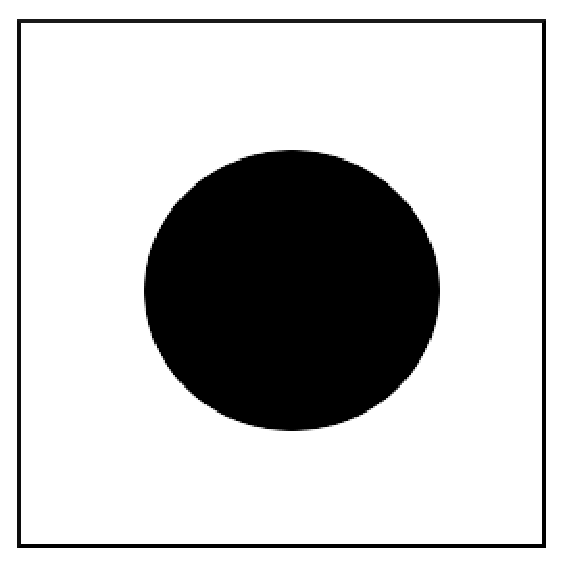
\includegraphics[scale=0.3]{images/circulo_250x250.eps}
\caption{Imagen artificial con bordes curvos entre clusters}
\label{fig:circulo}
\end{figure}

Las primeras pruebas para esta imagen consideran centroides iniciales aleatorios, y se trabajó nuevamente utilizando sólo las intensidades de gris primero y posteriormente incorporando las coordenadas de cada punto.

Los resultados obtenidos sin información espacial demuestran que el algoritmo es capaz de agrupar los puntos de manera correcta en zonas cerradas cuando existe un fuerte contraste de intensidades entre la zona interior y la exterior (figura \ref{fig:circulo_aleatorio} a y b). Al incluir las coordenadas espaciales los resultados obtenidos son diferentes. Si bien se logra diferenciar con claridad la zona central del fondo en la imagen original, se observa que las probabilidades de los puntos pertenecientes al cluster cerrado son afectadas por la distancia al centroide, que por lo que se puede observar, considerando que los puntos con valores de probabilidad más altos son los mas cercanos a éste, tiende a ubicarse en un punto tangente a la circunferencia (figura \ref{fig:circulo_aleatorio} c y d)

\begin{figure}[h]
\centering
\includegraphics[scale=0.08]{images/circulo-001.jpg}
\caption{Mapas de pertenencia con centroides iniciales aleatorios. (a - b)  sin información espacial (c - d) con información espacial.}
\label{fig:circulo_aleatorio}
\end{figure}

En la primera representación con información espacial (figura \ref{fig:circulo_aleatorio} - c) se puede ver que el rango de probabilidades para la zona circular varía desde $0,5$ tendiendo a $1$, pero sin lograr probabilidades altas, y en la segunda imagen (figura \ref{fig:circulo_aleatorio}-d) abarca probabilidades menores a $0.5$, pero no hay probabilidades nulas. A partir de la variación de colores que representan el mapa probabilístico, se observa claramente que hay incertidumbre para identificar los puntos pertenecientes a la región cerrada, y que esta incertidumbre aumenta en el resto de la imagen. Se puede apreciar además cómo las probabilidades en el fondo prácticamente recorren el rango completo, lo cual indica que la zona de fondo tampoco  es identificada con certeza como perteneciente a ningún cluster.

Luego se consideró la elección manual de los centroides iniciales: para uno de los clusters se ubicó en la zona central del círculo, mientras que para el otro fue seleccionado en el punto superior izquierdo de la imagen. No se evidencian diferencias en los resultados, y al igual que en el caso aleatorio, cuando se incluye información espacial los valores límites de probabilidades se desplazan hacia un punto tangente del objeto cerrado (figura \ref{fig:circulo_aleatorio_centr_manual}).

\begin{figure}[h]
\centering
\includegraphics[scale=0.08]{images/circulo-001.jpg}
\caption{Matriz de pertenencia, con centroide seleccionado manualmente. (a-b) sin información espacial. (c-d) con información espacial}
\label{fig:circulo_aleatorio_centr_manual}
\end{figure}

Al advertir que el resultado final era el mismo que con los centroides aleatorios,  se realizó el experimento de ejecutar el algoritmo con los centroides elegidos a mano pero con un límite de iteraciones acotado para observar cómo se desplazaban los mismos conforme las iteraciones avanzan. Como se aprecia en la figura \ref{fig:circulo_iteraciones}, inicialmente la circunferencia tiene valores cercanos a $0\%$ de pertenencia (figura \ref{fig:circulo_iteraciones}-a), pero los mismos aumentan a medida que se ejecutan más iteraciones, hasta llegar al resultado final (figura \ref{fig:circulo_iteraciones}-e), que coincide con el presentado en la figura \ref{fig:circulo_aleatorio_centr_manual}. A medida que el algoritmo progresa, el centroide se desplaza hacia un punto del borde de la circunferencia. También se puede ver que la región del fondo no logra ser identificada por el algoritmo, ya que las probabilidades abarcan el rango completo de 0 a 1. 

\begin{figure}[h]
\centering
\includegraphics[scale=0.08]{images/circulo_iteraciones_x1.jpg}
\caption{Matriz de pertenencia al primer cluster, con información espacial y selección manual de centroides iniciales. (a)Luego de 1 iteración, (b) luego de 10 iteraciones, ( c) luego de 25 iteraciones, (d) luego de 50 iteraciones, (e) luego de 100 iteraciones}
\label{fig:circulo_iteraciones}
\end{figure}

\subsection{Imágenes con ruido}
La siguiente serie de experimentos considera imágenes con ruido sal y pimienta. En la primera evaluación se utilizó una imagen con 1\% de ruido y luego se elevó al 30\% (figura \ref{fig:mitad_mitad_ruido_1p}).

\begin{figure}[H]
\centering
\includegraphics[scale=0.06]{images/original_mitad_con_ruido_1y30.jpg}
\caption{Ruido sal y pimienta 1\%}
\label{fig:mitad_mitad_ruido_1p}
\end{figure}

En caso de no incluir las coordenadas espaciales, los puntos de ruido son clasificados con una probabilidad baja de pertenencia a su clúster, debido a la diferencia de intensidad (figura \ref{fig:ruido_1y30}-a). El efecto se profundiza cuando analizamos una imagen con mayor presencia de ruido (figura \ref{fig:ruido_1y30}-b).


\begin{figure}[h]
\centering
\includegraphics[scale=0.055]{images/mitad_mitad__ruido_1y_30.jpg}
\caption{Matriz de pertenencias del cluster 1, sin información espacial. (a) con 1\% de ruido, (b) con 30\% de ruido
}
\label{fig:ruido_1y30}
\end{figure}

Contrariamente, cuando se añaden las coordenadas espaciales como otra característica al algoritmo, se obtiene una distribución general de probabilidades similar a la lograda para la imagen sin ruido (Figura \ref{fig:mitad_mitad_ruido_zoom} b-1), y al igual que en el experimento sin información espacial, los puntos con ruido son clasificados con menor probabilidad. 
En este caso, si comparamos en detalle las probabilidades obtenidas con y sin la información espacial, podemos observar que la probabilidad de pertenencia de los  puntos con ruido es más acertada cuando se utilizan las coordenadas del punto como característica adicional (Figuras \ref{fig:mitad_mitad_ruido_zoom} a-2 y b-2).


\begin{figure}[H]
\centering
\includegraphics[scale=0.05]{images/mitad_mitad_ruido_zoom-001.jpg}
\caption{Matriz de pertenencia al cluster 1, de la imagen con 1\% de ruido. 
(a-1) sin información espacial (a-2) acercamiento de región marcada en (a-1)
(b-1) con información espacial (b-2) acercamiento de región marcada en (b-1)}
\label{fig:mitad_mitad_ruido_zoom}
\end{figure}

\subsection{Imágenes con bias}
En las siguientes pruebas utilizamos una imagen con 3 regiones, correspondientes al fondo y a un objeto circular y un anillo alrededor del mismo que presentan bias (figura \ref{fig:circulo_bias}). El bias es una distorsión de la imagen causada por el instrumento de captura. Esta distorsión se presenta generalmente sobre los bordes de los objetos y causa cambios en la intensidad de los píxeles, de manera que el mismo tejido es representado por diferentes valores en la imagen \citep{juntu2005bias}.

\begin{figure}[H]
\centering
\includegraphics[scale=0.3]{images/biasing.png}
\caption{Imagen de bordes curvos con 3 clusters y bias}
\label{fig:circulo_bias}
\end{figure}

El comportamiento del algoritmo cuando no se utilizan coordenadas espaciales es similar al observado en las pruebas anteriores, las tres zonas fueron correctamente detectadas y se puede notar como el bias afecta las probabilidades de las zonas debido al cambio de intensidades  (figura \ref{fig:matriz_circulo_bias}).

\begin{figure}[H]
\centering
\includegraphics[scale=0.3]{images/bias_sin_coord.jpg}
\caption{Mapas de pertenencia sin información espacial (a) fondo (b) anillo ( c) centro}
\label{fig:matriz_circulo_bias}
\end{figure}

Cuando utilizamos coordenadas espaciales para la clasificación de esta imagen, podemos apreciar que, al igual que en los experimentos anteriores, el algoritmo no detecta correctamente la zona del fondo (figura \ref{fig:matriz_circulo_bias_espacial} a y b). En el caso particular de la imagen para el clúster del centro (figura \ref{fig:matriz_circulo_bias_espacial} - c), vemos concretamente la influencia de las coordenadas espaciales, ya que la zona central y el anillo que la rodea son reconocidos prácticamente como un solo grupo, pese a la diferencia de intensidades.

\begin{figure}[H]
\centering
\includegraphics[scale=0.3]{images/bias_con_coord.jpg}
\caption{Mapas de pertenencia con información espacial (a) cluster del fondo, zona izquierda (b) cluster del fondo, zona derecha  (c) centro}
\label{fig:matriz_circulo_bias_espacial}
\end{figure}

\subsection{Imágenes con bias y ruido}

En nuestra última prueba utilizamos una imagen con bias y ruido. En esta situación, la clusterización resultante es de menor calidad que en los experimentos anteriores debido a la presencia de una alto porcentaje de ruido así como un biasing pronunciado. 

\begin{figure}[H]
\centering
\includegraphics[scale=0.3]{images/biasing_con_ruido.png}
\caption{Imagen con bias y ruido}
\label{fig:circulo_bias_ruido}
\end{figure}

En los mapas de pertenencia de la figura \ref{fig:circulo_bias_ruido_cluster} se puede apreciar que, pese al ruido y al bias, el fondo de la imagen es correctamente clasificado (figura \ref{fig:circulo_bias_ruido_cluster}-a), pero en el segundo y tercer mapa el anillo y la parte central de la imagen original no son claramente distinguidos (figura \ref{fig:circulo_bias_ruido_cluster} b y c). Las pertenencia de la zona central y el anillo varían entre 0 y 1 y además se mezclan en determinadas zonas.

\begin{figure}[H]
\centering
\includegraphics[scale=0.3]{images/bias_sin_coord_con_ruido.jpg}
\caption{Mapa de pertenencia sin información espacial (a) cluster del  fondo (b) centro 1 (c) centro 2}
\label{fig:circulo_bias_ruido_cluster}
\end{figure}

\subsection{Análisis de costo y convergencia}
En todos los casos analizados, la curva de convergencia de la función costo tiene la forma mostrada en la Figura 17. Siempre hay un periodo inicial con un valor alto de la función costo y luego un punto de inflexión a partir del cual desciende abruptamente y los valores oscilan levemente hasta que el algoritmo se detiene, como se mencionó en la sección \ref{Introduccion}.

\begin{figure}[h]
\centering
\includegraphics[scale=0.3]{images/FALTA.png}
\caption{Curva de convergencia}
\label{fig:convergencia}
\end{figure}


\section{Extracción de mallas}\label{section:extraccion_de_mallas}
Para obtener una superficie cerrada que se pueda utilizar como entrada para el algoritmo de Modelos Deformables, es necesario extraer el contorno del objeto de interés a partir de las matrices de probabilidades que se obtuvieron utilizando el algoritmo de Fuzzy C-Means. En la Figura \ref{fig:pipe_obtencion_malla} se pueden observar los pasos que se realizan para obtener esta malla. En primer lugar, se realiza un umbralado de los mapas probabilísticos a fin de obtener volúmenes binarios que incluyan aquellos puntos que pertenecen a cada región de interés. Posteriormente, se aplica un algoritmo de rellenado de huecos y de limpieza de ruido para reducir posibles perturbaciones que puedan generar mallas discontinuas o con objetos aislados. Finalmente, se extrae una malla de superficie a partir del contorno de cada volumen.

\begin{figure}[H]
	\centering
	\includegraphics[scale=0.4]{images/pipeline_de_obtencion_de_malla.jpg}
	\caption{Pipeline de obtención de malla}
	\label{fig:pipe_obtencion_malla}
\end{figure}

En las siguientes secciones se detalla cada una de estas operaciones.

\subsection{Umbralado}\label{section:umbralado}
El primer paso es realizar un umbralado de los mapas probabilísticos, con el objeto de obtener c volúmenes binarios (uno por cada cluster) indicando si cada punto pertenece o no al cluster asociado al mismo. Para lograr esto, el método evalúa cada punto de la imagen, comparando las probabilidades del punto en las matrices de probabilidades obtenidas por Fuzzy C-Means, y asignándolo a aquel cluster que presente mayor probabilidad. En caso de que exista igualdad de probabilidades, se decidió tomar el cluster que haya sido evaluado primero.

Como se puede observar en la Figura \ref{fig:umbralado}, el umbralado aplicado al mapa de probabilidades donde se ve en tonos rojos las probabilidades altas de pertenencia y en tonos azules las probabilidades bajas, resulta en un volumen binario, donde en blanco se representa el objeto de interés y en negro lo que no pertenece a éste.

\begin{figure}[H]
	\centering
	\includegraphics[scale=0.3]{images/umbralado.png}
	\caption{Umbralado del mapa de probabilidades}
	\label{fig:umbralado}
\end{figure}


\subsection{Rellenado de huecos}
En algunos casos, luego del umbralado prevalecen pequeños huecos dentro del volumen binario. Para que el algoritmo de mallado no extraiga una superficie de estas zonas no deseadas, eliminamos los pequeños huecos que quedaron dentro del área de interés. Aplicamos un método de eliminación de huecos que consiste en marcar como pertenecientes a la zona de interés aquellos grupos de voxeles que hayan sido previamente asignados al fondo pero que no están conectados al mismo \citep{soille2003morphological}. Para estudiar la conexión con el fondo se realizó un recorrido del volumen binario desde el fondo hacia la región de interés.

\begin{figure}[H]
	\centering
	\includegraphics[scale=0.5]{images/rellenado.png}
	\caption{En rojo, el grupo de vóxeles contiguos rellenados (mismo voxel en los cortes axial, coronal y sagital)}
	\label{fig:rellenado}
\end{figure}

En la Figura \ref{fig:rellenado} exponemos un ejemplo de rellenado. Pese a que son pocos puntos los corregidos por el rellenado, este es necesario para evitar que el algoritmo de extracción de mallas triangule esas pequeñas áreas.

\subsection{Extracción de la malla}
El último paso es obtener el contorno del objeto de interés en forma de una lista de puntos vinculados. Estos puntos se obtienen a partir del volumen binario utilizando un enfoque de simplificación de superficie \citep{fang2009tetrahedral}, que permite obtener una malla que vincula los puntos mediante triángulos. Inicialmente se obtiene una representación de la superficie desde el volumen tridimensional. Esto se logra identificando cuando hay un cambio de blanco a negro o de negro a blanco en el volumen binario. Una vez obtenida esta información, se procede a generar una lista de puntos y una lista de triplas de puntos que representan cada triángulo.


\section{Modelos deformables}\label{section:modelos_deformables}
El esquema de segmentación propuesto contempla la utilización de Modelos Deformables (Superficies Activas) para mejorar la segmentación, mediante la integración de información espacial a la aproximación inicial obtenida con el algoritmo de Fuzzy C-Means. El objetivo es obtener una superficie cerrada y suave, que logre ajustarse lo más posible a las estructuras de interés.

Inicialmente se describen las características del modelo clásico de Contornos Activos en 2D \citep{kass1988snakes} (Sección \ref{section:modelo_continuo_contornos_activos}). Luego se presenta su aproximación numérica discreta en 2D y 3D (Sección \ref{section:modelo_discreto_contornos_activos}), propuesta por \cite{mcinerney2000t} y considerada en este trabajo. Por último, se incorpora un análisis de sensibilidad para mostrar el comportamiento de los diferentes parámetros del algoritmo (Sección \ref{section:estudio_de_sensibilidad}).

\subsection{Modelo continuo de Contornos Activos en 2D}\label{section:modelo_continuo_contornos_activos}

En el esquema original de Contornos Activos en 2D se busca definir un contorno, conocido como Snake, que delimita a la región de interés. Matemáticamente, un Snake se define como una curva paramétrica (Figura \ref{fig:curva_parametrica}):

%
\begin{equation}	
	v(s) = (x(s), y(s)), s \in [0,1]
\end{equation}
%


\begin{figure}[H]
	\centering
	\includegraphics[scale=0.05]{images/grafico_snake_parametrico.jpg}
	\caption{Curva paramétrica}
	\label{fig:curva_parametrica}
\end{figure}

Esta curva se desplaza sobre el espacio de la imagen, a partir de su posición inicial, mediante la acción de una serie de fuerzas internas y externas, con el objetivo de minimizar un funcional de energía asociada $E$ (Ecuación \ref{eq:Ecx}). Este funcional está definido por dos componentes: una energía interna que controla las características intrínsecas de la curva, las cuales definen la deformación y capacidad de adaptarse al objeto de interés; y una energía externa, que guía o “empuja” esta curva, basándose en información extraída a partir de la imagen:


%
\begin{equation}
	E(v) = E_{int}(v) + E_{ext}(v)
\label{eq:Ecx}
\end{equation}
%


La energía interna restringe la deformación de la curva, y está dada por:

%
\begin{equation}
E_{int}(v) = \int_{0}^{1} w_{1}(s) \left| \dfrac{\delta v}{\delta s} \right|^{2} + w_{2}(s) \left|\dfrac{\delta^{2}v}{\delta s^2} \right|^{2} ds
\end{equation}
%
La primera componente se asocia a la energía de tensión, que es la que controla el estiramiento y hace que el contorno se comporte como una cuerda. La segunda componente introduce características de rigidez a la curva, asegurando la obtención de un contorno suave. Los parámetros no negativos $w_{1}(s)$ y $w_{2}(s)$ determinan el nivel de tensión y rigidez del contorno, respectivamente. Al variar estos coeficientes, la curva puede cambiar su comportamiento durante la evolución: si se establece un valor 0 para uno o ambos parámetros en un punto s, se permitirá discontinuidad en ese punto. Estos parámetros pueden depender de s si se pretende que la tensión/flexión varíe en ciertos puntos de la curva, aunque en la práctica se les suele asociar valores constantes.

Por otro lado, la energía externa está dada por:
%
\begin{equation}
	E_{ext}(v) = \int_{0}^{1} P(v(s))ds
\end{equation}
%
y representa la energía potencial del modelo, definida a partir de un campo de potenciales $P$ que se diseñan de forma tal que sus mínimos locales coincidan con extremos de los elementos de interés (intensidad, bordes u otra característica de la imagen que resulte relevante para el dominio del problema). De este modo se busca poder delimitar la superficie de interés lo más correctamente posible. Generalmente, los bordes presentes en la imagen actúan como atractores del contorno, pudiendo detener la expansión provocada por las fuerzas aplicadas. De manera similar, y mediante el uso de algún criterio específico de homogeneidad, es posible forzar que la curva se expanda en regiones con propiedades similares, y que detenga su avance cuando esta homogeneidad se interrumpe (por ejemplo, ante la presencia de bordes).
La forma del contorno alcanzará su estado final cuando las fuerzas internas y externas se equilibren, minimizando $E$.

\subsection{Modelo discreto de Contornos Activos}\label{section:modelo_discreto_contornos_activos}
Las ecuaciones definidas en el modelo continuo no poseen una solución analítica, por lo que es necesario aplicar métodos numéricos para obtener una aproximación. Para esto, se busca discretizar el modelo en espacio y tiempo, muestreando la curva o superficie a intervalos regulares y considerando alguna representación discreta del mismo.

Una posible discretización es la que se propone en \citep{mcinerney2000t}. Para trabajar en 2 dimensiones, se define un contorno cerrado bidimensional formado por $n$ nodos conectados en serie por $n$ arcos (Figura \ref{fig:modelo_continuo_snakes}), donde se asocia a cada nodo una posición $s_{i}(t) = (x_{i}(t),y_{i}(t))$, junto a un vector normal y las componentes de fuerza que actúan sobre él, estableciendo además la condición de frontera $s_{0}(t)=s_{n}(t)$ para garantizar una curva cerrada.

\begin{figure}[H]
	\centering
	\includegraphics[scale=0.6]{images/ovalo_continuo_vs_discreto.jpg}
	\caption{(a) Modelo continuo de Snakes. (b) Aproximación discreta del modelo}
	\label{fig:modelo_continuo_snakes}
\end{figure}

Partiendo de esta representación discreta en 2 dimensiones, resulta sencillo extender la definición para incorporar una tercera dimensión. Así, en el modelo 3D discreto se utiliza, en lugar de una curva, una malla elástica cerrada que se comporta como una membrana o superficie deformable. Esta malla está compuesta por un conjunto de nodos vinculados por triángulos. A cada nodo o vértice de la malla se le asocia una posición $s_{i}(t)=(x_{i}(t),y_{i}(t), z_{i}(t))$, variable en el tiempo, junto a un vector normal y las componentes de fuerza que actúan sobre él.

La superficie activa evoluciona mediante desplazamientos de sus nodos $s_{i}$, a través de la ecuación de movimiento de Lagrange:

%
\begin{equation}
\gamma_{i}s_{i} - a\alpha_{i}(t) + b\beta_{i}(t) = c\rho_{i}(t) + df_{i}(t)
\end{equation}
%
donde $\alpha$, $\beta$, $\rho$  y $f$ son magnitudes vectoriales que representan las fuerzas de tensión, flexión, inflación y gradiente, respectivamente, y $\gamma_{i}$ es un coeficiente de amortiguación que regula la velocidad $s_{i}$ del $i$-ésimo nodo.

La energía interna permite que el modelo se comporte como una membrana elástica, donde la fuerza de tensión restringe el estiramiento de la superficie, mientras que la fuerza de flexión representa la resistencia a deformaciones de curvatura. Por otro lado, la energía externa guía a la malla hacia los bordes de la región de interés, donde la fuerza de inflación actúa en dirección al vector normal, inflando o desinflando dependiendo de la similitud con alguna característica de la región en el vértice, mientras que la fuerza de gradiente actúa en dirección opuesta al vector normal, para detener el avance de la malla al acercarse a los bordes. 

La superficie detiene su deformación cuando ningún desplazamiento individual excede un cierto error de convergencia, o cuando se alcanza un número máximo de pasos preestablecidos.

El modelo discreto utilizado en nuestra implementación se basa en el planteado por \citep{mcinerney2000t}, que propone utilizar el método de integración explícito de Euler, aproximando de esta forma una solución numérica a la Ecuación Diferencial de la siguiente forma:

%
\begin{equation}
S^{(t+\Delta t)}_{i} = S_{i}^{t} - \Delta t.\gamma(a\alpha_{i}^{t} + b\beta_{i}^{t} - c\rho_{i}^{t} - df_{i}^{t})
\end{equation}
%
Como se describió anteriormente, el algoritmo de deformación se inicializa con una malla obtenida a partir del volumen segmentado mediante el método de Fuzzy C-Means y se aplica iterativamente hasta alcanzar la convergencia del modelo. Para realizar la deformación, en cada paso se obtienen las fuerzas (tensión, flexión, inflación y gradiente) sobre cada vértice de la malla, realizando una interpolación trilineal. En particular, para obtener la fuerza de inflación, se calculan además los vectores normales a la superficie en cada vértice. 

Por último, se aplican todas las fuerzas a cada vértice de la malla, ponderándolas en función de los parámetros de calibración ($a$, $b$, $c$ y $d$) para obtener la nueva posición de la malla, se incrementa la cantidad de pasos y se verifica el criterio de finalización.

El pseudocódigo del procedimiento usado se puede ver en el Pseudocódigo \ref{alg:modelos_deformables}.

\begin{program}
\begin{verbatim}

Mientras steps < MAX_STEPS O NO haya convergencia
  - Calcular la fuerza de tensión para todos los vértices
  - Calcular la fuerza de flexión para todos los vértices
  - Obtener el vector normal en todos los vértices (ponderado por 
      los vectores normales de los triángulos adyacentes)
  - Calcular la fuerza de inflación para todos los vértices
  - Obtener el vector gradiente para todos los vértices
  - Calcular la fuerza de gradiente para todos los vértices
  - Actualizar la posición de todos los vértices, aplicando las 
      fuerzas calculadas, y ponderando con los coeficientes de calibración.
\end{verbatim}
\caption{Pseudocódigo de Modelos deformables}
\label{alg:modelos_deformables}
\end{program}

En las siguientes subsecciones se explica en detalle las consideraciones tenidas en cuenta para la implementación de las diferentes fuerzas.

\subsubsection{Energía interna}\label{section:energia_interna}
Como se explicó para el modelo continuo, la energía interna brinda al modelo las características de deformación de una membrana elástica. Los términos $\alpha_{i}$ y $\beta_{i}$ de la ecuación diferencial se corresponden a la fuerza de tensión y flexión. La primera representa la resistencia de la superficie al estiramiento, e intenta preservar una distancia uniforme entre los nodos, mientras que la fuerza de flexión representa la resistencia a la deformación de la curvatura, lo que permite generar una superficie suave. Ambas fuerzas se aplican sobre cada vértice i de la malla, y se calculan a partir del operador Laplaciano y Laplaciano cuadrático, como aproximación a la segunda y cuarta derivada respecto de la posición de vértice \citep{mcinerney2000t}. Para aproximar la derivada para calcular la \emph{fuerza de tensión}, se utiliza el operador “sombrilla”, tomando en cuenta la topología de una malla local alrededor del vértice $i$, a partir de la siguiente ecuación:

%
\begin{equation}
\alpha_{i}(t) = \dfrac{1}{m}\sum_{j\in N(i)} s_{j}(t) - s_{i}(t)
\end{equation}
%
donde $N_{i}$ representa al conjunto de vértices $s_{j}$ vecinos al vértice $s_{i}$, y $m$ es el número de vértices  vecinos.

En el caso de la \emph{fuerza de flexión}, el Laplaciano cuadrático puede aproximarse nuevamente aplicando el operador “sombrilla”, pero en este caso se aplica sobre los valores de la fuerza de tensión en cada vértice, resultando:

%
\begin{equation}
\beta_{i}(t) = \dfrac{1}{m} \sum_{j\in N(i)} \alpha_{j}(t) - \alpha_{i}(t)
\end{equation}
%
\subsubsection{Energia externa}\label{section:energia_externa}
La energía externa es la que guía a la malla hacia la frontera de la región de interés, y está formada por las fuerzas de inflación y de gradiente, que en la ecuación diferencial se representan con los términos $\rho_{i}$ y $f_{i}$, respectivamente.

La \emph{fuerza de inflación} se aplica para empujar la superficie hacia los bordes de la imagen y se describe como: 

%
\begin{equation}
\rho_{i}(t) = F(I(s_{i}(t))) n_{i}(t)
\end{equation}
%
donde $n_{i}$ es el vector normal unitario a la superficie para el nodo $i$, mientras que $F(I(s_{i}))$ es una función binaria que relaciona $i$ al campo de intensidades de la imagen $I$. La implementación más sencilla de la función $F$ vincula directamente a la fuerza con la intensidad de la imagen de la siguiente forma:

%
\begin{equation}
F(I(s)) = \begin{cases} 1 & \text{si } I(s) \geq T \\ -1 & \text{en otro caso} \end{cases}
\end{equation}
%
siendo $T$ un umbral definido sobre las intensidades de la imagen. Esta función $F$ hace que la malla se contraiga cuando la intensidad del vértice es menor al umbral $T$.

Para evitar que el modelo sea afectado por el ruido y se filtre a través de otras regiones, se puede incorporar estadística sobre las intensidades de la región considerada \citep{ivins1994statistical} definiendo la función $F$ como:

%
\begin{equation}
F(I(s)) = \begin{cases} 1 & \text{si } \left|I(s) - \mu \right| \leq k\sigma \\ -1 & \text{en otro caso} \end{cases}
\end{equation}
%
donde $\mu$ y $\sigma$ corresponden a la media y al desvío estándar de las intensidades de la región de interés, y $k$ es una constante definida.

En la presente implementación se utiliza esta definición de fuerza, pero para enriquecerla aprovechando la información obtenida por Fuzzy c-Means (que permite incorporar múltiples descriptores extraídos a partir de la imagen), en lugar de definirla sobre $I(s)$, la misma está definida sobre el campo escalar de probabilidades $\rho(s)$ asociado a la región de interés, resultando en:

%
\begin{equation}
F(P(s)) = \begin{cases} 1 & \text{si } \left|\rho(s) - \mu_{p} \right| \leq k\sigma_{p} \\ -1 & \text{en otro caso} \end{cases}
\end{equation}
%
donde $\rho(s)$ es una función que asocia a cada nodo $s$ con su probabilidad de acuerdo al mapa probabilístico obtenido como resultado del método Fuzzy c-Means, $\mu_{p}$ la media de las probabilidades dentro de la región de interés, y $\sigma_{p}$ el desvío estándar de estas probabilidades en la región.

Para detener el avance del modelo ante bordes bien marcados, se incluye la \emph{fuerza de gradiente}, que se define como:

%
\begin{equation}
f_{i}(t) = \nabla P(s_{i}(t))
\end{equation}
%
donde $\nabla$ es el operador gradiente y la fuerza potencial $P$ describe como:

%
\begin{equation}
P(s) = - \left\| \nabla(G_{\sigma} * I(s)) \right\| 
\label{eq:zz}
\end{equation}
%
donde $G_{\sigma} * I(s)$ denota una distribución Gaussiana de suavizado de la imagen con desviación estándar $\sigma$ [mcinerney2000t].

En este trabajo, al igual que para la fuerza de inflación, en lugar de estudiar el gradiente sobre $I(s)$, el mismo se obtiene sobre $p(s)$:

%
\begin{equation}
P(s) = - \left\| \nabla(G_{\sigma} * p(s)) \right\|
\end{equation}
%
Así, el gradiente ahora representa variaciones abruptas en las probabilidades. El suavizado gaussiano se mantiene con el objetivo de resolver discontinuidades en las probabilidades que puedan estar asociadas a la presencia de ruido.

\subsection{Estudio de sensibilidad}\label{section:estudio_de_sensibilidad}
Dado que el algoritmo de Modelos deformables depende de múltiples parámetros, es necesario comprender cómo afectan los valores de cada uno de ellos de manera que la calibración de los mismos pueda realizarse más sistemáticamente y sea posible obtener resultados más precisos. Esta sección tiene por objetivo atender esta necesidad, brindando una serie de contribuciones experimentales a ese respecto. Durante el estudio se dejaron fijos todos los parámetros del modelo excepto uno, al que se varió de manera aislada para estudiar el comportamiento resultante. Este análisis fue realizado sobre el segmento correspondiente a la materia blanca de una imagen MRI artificial, aunque puede extrapolarse hacia otros tejidos en otros tipos de imágenes.

\subsubsection{Cantidad de pasos y error de convergencia}
La cantidad de pasos hace referencia a la cantidad de iteraciones del método de integración de Euler necesarios para la resolución de la ecuación diferencial que define el comportamiento de la superficie activa. Es de esperar que, luego de un cierto número de iteraciones, el método converja y no existan grandes cambios en la solución. Así, es posible definir un error de convergencia $\epsilon$ experimentalmente, tal que el mismo represente el mínimo desplazamiento promedio tolerado para los nodos de la malla. Cuando dos sucesivas iteraciones alteran las posiciones de los vértices en un promedio inferior al dado por el error $\epsilon$, se asume que el modelo converge y se retorna la solución. El desplazamiento promedio se obtiene calculando la media de las normas euclídeas de los vectores de desplazamiento en cada iteración, para cada nodo que compone la malla que está siendo deformada.

Dado que en el esquema propuesto el algoritmo de Modelos Deformables se inicializa con una malla cercana a los bordes de la región de interés, se espera que el número de iteraciones necesario para que el modelo alcance la convergencia no sea excesivamente grande. En la Figura \ref{fig:convergencia_snakes} se ilustra la evolución del desplazamiento promedio de los nodos, respecto a la cantidad de pasos de integración. Como puede observarse, el desplazamiento promedio cae abruptamente en las primeras iteraciones, hasta que se estabiliza con un cierto error de convergencia.

\begin{figure}[H]
	\centering
	\includegraphics[scale=0.8]{images/convergencia_snakes.jpg}
	\caption{Evolución del desplazamiento promedio respecto de la cantidad de iteraciones}
	\label{fig:convergencia_snakes}
\end{figure}

\subsubsection{Coeficientes de las fuerzas internas}
Los coeficientes $a$ y $b$, que ponderan a las fuerzas de tensión y flexión respectivamente, son
los que controlan la rigidez de la superficie activa. Es de esperar que cuando toman valores altos, la superficie sea más resistente a las deformaciones que con valores pequeños. 

En la Figura \ref{fig:sensibilidad4} se presenta el corte axial de tres superficies diferentes, obtenidas éstas fijando los parámetros $c=0.15$, $d=1.5$ y $k=2$, variando únicamente el valor de $a$ y $b$ (en particular, $a=b=0.005, 0.5 \text{ y } 1$).

\begin{figure}[H]
	\centering
	\includegraphics[scale=0.05]{images/sensibilidad4.jpg}
	\caption{Corte de diferentes superficies activas obtenidas con valores de $c=0.15$, $d=1.5$ y $k=2$ fijos, $a = b = 0.005$ (amarillo), $0.5$ (naranja) y $1$ (rojo). }
	\label{fig:sensibilidad4}
\end{figure}

Como se puede observar en la Figura \ref{fig:sensibilidad4}, la malla generada con valores bajos de $a$ y $b$ (amarilla) se adapta mejor a las concavidades y convexidades de la imagen de referencia, pero a su vez, se puede observar en el acercamiento, que es menos suave y que en algunas zonas la malla se deforma, contrayéndose sobre sí misma. A medida que se incrementan los valores de estos parámetros, las superficies resultan más suaves pero dejan de adaptarse a las concavidades y convexidades más pronunciadas (mallas naranja y roja). 

\subsubsection{Coeficientes de la fuerza de inflación}
La fuerza de inflación depende de dos parámetros. El parámetro k, que determina el nivel de permisividad, definiendo si la fuerza va a empujar o contraer la malla. Por otro lado,  el coeficiente c que acompaña a la fuerza de inflación, define  cuánto influye en la evolución de la superficie activa. Es de esperar que, cuanto más alto sea su valor, la superficie activa tienda a inflarse o desinflarse con mayor velocidad.

Para evaluar el comportamiento de la malla, según el valor de k, en la Figura \ref{fig:sensibilidad8} podemos observar el corte axial de tres mallas generadas fijando los parámetros $a=b=0.08$, $c=0.15$ y $d=1.5$, variando $k$ con valores $0.5, 2 y 4$.

\begin{figure}[H]
	\centering
	\includegraphics[scale=0.05]{images/sensibilidad8.jpg}
	\caption{Corte de diferentes superficies activas obtenidas con valores $a=b=0.08$, $c=0.15$ y $d=1.5$ fijos,  $k$ de $0.05$ (amarillo), $2$ (naranja) y $4$ (rojo). }
	\label{fig:sensibilidad8}
\end{figure}

Se puede observar que la malla roja, con un valor alto de k, se infló sobre valores bajos de probabilidad, mientras que las mallas con valores más bajos (amarilla y naranja) se mantienen más cercanas a las probabilidades altas de la región.

Por otro lado, en la Figura \ref{fig:sensibilidad6}, se puede apreciar el corte coronal de tres mallas generadas fijando los valores $a=b=0.08$, $d=1$ y $k=4$,  variando los valores de $c$ con $0.05$, $0.2$ y $0.5$.

\begin{figure}[H]
	\centering
	\includegraphics[scale=0.05]{images/sensibilidad9.jpg}
	\caption{(a)Corte de diferentes superficies activas obtenidas con valores de $a=b=0.08$, $d=1$ y $k=4$ fijos, $c$ de $0.05$ (amarillo), $0.2$ (naranja) y $0.5$ (rojo). (b) y ( c) Acercamientos en diferentes zonas del corte}
	\label{fig:sensibilidad9}
\end{figure}

En general, la malla asociada a un valor alto de  $c$ (roja) es más amplia que las mallas obtenidas con valores más bajos (naranja y amarilla). Esto se debe a que se utilizó un valor de $k$ alto, permitiendo que la malla se infle ante mayor variación de probabilidades. En particular, en el acercamiento (b) se puede ver cómo a medida que el valor de c aumenta, la malla se infla más sobre la convexidad que se observa con baja probabilidad. Sin embargo, si observamos el acercamiento (c), donde hay una concavidad con algunos puntos con probabilidades muy bajas, se puede ver que la malla roja se contrajo más que las de valores bajos de $c$ (mallas amarilla y naranja), ya que en este punto, la función $F(p(s))$ indicó que debía contraerse.

\subsubsection{Coeficiente de la fuerza gradiente}
El parametro $d$ influye sobre la fuerza de gradiente. En la Figura \ref{fig:sensibilidad6} se presenta un corte axial de cuatro mallas generadas con valores fijos de $a=b=0.08$, $c=0.15$ y $k=4$ y variando los valores de $d$ con $0.5$ (verde), $1$ (amarillo), $4$ (naranja) y $10$ (rojo).

\begin{figure}[H]
	\centering
	\includegraphics[scale=0.05]{images/sensibilidad6.jpg}
	\caption{(a) Corte de diferentes superficies activas obtenidas con valores de $a=b=0.08$, $c=0.15$ y $k=4$ fijos, $d$ $0.5$ (verde), $1$ (amarillo), $4$ (naranja) y $10$ (rojo). (b) y ( c) Acercamientos en diferentes zonas del corte}
	\label{fig:sensibilidad6}
\end{figure}

En este caso la malla obtenida con un valor alto de $d$ (roja) se mantiene más contraída sobre los bordes de la imagen, y a medida que se reduce este valor (mallas naranja, amarilla y verde) se aleja de estos. En el acercamiento (b), se puede ver que la malla verde, con valor muy bajo de $d$, se escapa alejándose mucho del borde de la imagen. Por otro lado, en el acercamiento (c) la malla roja con valor muy alto de $d$, no pudo avanzar sobre la convexidad, mientras que con valores más bajos (mallas verde, amarilla y naranja), se observa que las mallas se fueron adaptando a esta forma.
